\section{Conformità normativa e valutazione d'impatto}\label{sec:conformita}

Questa sezione colloca il sistema nel quadro normativo che si applica a una struttura sanitaria italiana e ne valuta l'impatto sulla protezione dei dati. Le scelte tecniche delle sezioni precedenti vengono qui ricondotte agli obblighi da cui discendono, e i rischi che restano sono stimati con un metodo dichiarato e ripetibile.

\subsection{Quadro normativo e ruoli}
Il sistema tratta dati relativi alla salute, una categoria particolare di dati personali (art.~9 GDPR\cite{gdpr}), e quindi ricade nel GDPR e nel Codice in materia di protezione dei dati personali, come modificato per adeguarlo al regolamento\cite{codice-privacy}. Si applicano inoltre:
\begin{itemize}
  \item \textbf{la disciplina del Fascicolo Sanitario Elettronico} (art.~12 del d.l.~179/2012 e decreto del Ministero della salute del 7~settembre 2023\cite{dl179,dm-fse}). Il fascicolo viene alimentato senza consenso, mentre la sua \emph{consultazione} per finalità di cura richiede il consenso dell'interessato, che è sempre revocabile e non condiziona l'erogazione delle cure; tutte le operazioni sono registrate e il paziente può vedere chi ha consultato i suoi dati\cite{garante-fse}. È il modello seguito dal prototipo;
  \item \textbf{la direttiva NIS2} e il d.lgs.~138/2024 che la recepisce\cite{nis2,dlgs138}: i prestatori di assistenza sanitaria sono tra i settori ad alta criticità e devono adottare misure di gestione del rischio informatico e notificare gli incidenti significativi al CSIRT nazionale (paragrafo~\ref{sec:nis2});
  \item \textbf{le regole sui cookie} (art.~122 del Codice e linee guida del Garante\cite{garante-cookie}). L'applicazione usa un solo cookie tecnico di sessione, necessario al servizio, che non richiede consenso ma è descritto nell'informativa.
\end{itemize}

Il \textbf{titolare} del trattamento è la struttura sanitaria, che nomina un \textbf{responsabile della protezione dei dati} (RPD), obbligatorio per un ente pubblico che tratta su larga scala categorie particolari di dati (art.~37). Sono \textbf{responsabili del trattamento} ai sensi dell'art.~28 il fornitore dell'infrastruttura su cui gira il backend e il fornitore del nodo con cui il backend accede alla blockchain. Quest'ultimo riceve le transazioni, che contengono solo valori opachi, e l'indirizzo di rete del backend. Il wallet del paziente è invece uno strumento scelto e gestito dal paziente.

\subsection{Trattamenti e basi giuridiche}\label{sec:basi}
La tabella~\ref{tab:basi} riporta i trattamenti del sistema con le basi giuridiche. La scelta centrale riguarda il consenso. La tenuta della cartella e la cura si fondano su obblighi di legge e sull'art.~9(2)(h) GDPR, non sul consenso. Il consenso che il paziente firma con il wallet (sezione~\ref{sec:blockchain}) è invece l'\emph{autorizzazione alla consultazione} prevista per il Fascicolo Sanitario Elettronico: decide quale medico può leggere la cartella, per quale finalità e fino a quando. Così una revoca blocca la consultazione senza intaccare né l'obbligo di conservare la documentazione clinica né l'accesso nei casi di emergenza.

\begin{table}[H]
\centering\footnotesize
\renewcommand{\arraystretch}{1.2}
\begin{tabular}{@{}l p{.33\textwidth} p{.47\textwidth}@{}}
\toprule
& Trattamento & Base giuridica\\
\midrule
T1 & Tenuta della cartella clinica e referti firmati & Obbligo di legge e compito di interesse pubblico (art.~6(1)(c) ed (e)); diagnosi e cura (art.~9(2)(h) e 9(3), segreto professionale)\\
T2 & Consultazione della cartella da parte di un medico & Come T1, con il consenso alla consultazione del paziente previsto dalla disciplina del fascicolo sanitario, per finalità e con scadenza\\
T3 & Accesso d'emergenza & Interessi vitali dell'interessato che non può prestare il consenso (art.~6(1)(d) e 9(2)(c))\\
T4 & Registro degli accessi (sulla catena e cifrato) & Obbligo di sicurezza e di tracciamento degli accessi (art.~6(1)(c), art.~32, art.~5(2))\\
T5 & Autenticazione e gestione degli account & Obbligo di sicurezza del trattamento (art.~6(1)(c) e art.~32)\\
T6 & Consultazione per finalità di ricerca & Consenso esplicito dell'interessato (art.~9(2)(a) e 9(2)(j), art.~89 GDPR, art.~110 del Codice)\\
\bottomrule
\end{tabular}
\caption{Trattamenti del sistema e relative basi giuridiche. Il registro completo è nell'appendice~\ref{app:registro}.}\label{tab:basi}
\end{table}

\subsection{Principi e diritti degli interessati}
La tabella~\ref{tab:principi} collega ogni principio dell'art.~5 e ogni diritto degli interessati alla misura che lo attua.

\begin{table}[H]
\centering\footnotesize
\renewcommand{\arraystretch}{1.2}
\begin{tabular}{@{}p{.27\textwidth} p{.67\textwidth}@{}}
\toprule
Principio o diritto & Attuazione nel sistema\\
\midrule
Liceità e trasparenza & Informativa versionata, servita dal backend e mostrata prima della firma; versione e impronta SHA-256 dell'informativa entrano nel consenso firmato, che prova quale testo il paziente ha letto\\
Limitazione della finalità & Consenso distinto per cura, ricerca e amministrazione; l'accesso è concesso solo per la finalità dichiarata dal medico e coperta dal consenso\\
Minimizzazione & Sulla catena solo ancore HMAC, impronte ed esiti; titoli e testi dei referti cifrati; un solo cookie tecnico\\
Esattezza & Rettifica per integrazione: un nuovo referto firmato, senza cancellare i precedenti (art.~16)\\
Limitazione della conservazione & Consensi con scadenza (al massimo un anno); sessioni con durata massima; cancellazione su richiesta per i dati non soggetti a obblighi di conservazione\\
Integrità e riservatezza & Passkey FIDO2, cifratura ibrida post-quantistica, firma dei referti, audit su blockchain (sezioni~\ref{sec:fido2}--\ref{sec:dati})\\
Responsabilizzazione & Registro dei trattamenti, valutazione d'impatto, audit verificabile da terzi, sorgente dei contratti verificato pubblicamente\\
\midrule
Accesso (art.~15) & Pagina \emph{I miei referti} e registro di chi ha consultato la cartella, verificabile sulla catena\\
Portabilità (art.~20) & Esportazione in JSON di referti, ricevute dei consensi e registro degli accessi\\
Revoca del consenso (art.~7(3)) & Revoca immediata dall'applicazione, registrata sulla catena\\
Cancellazione (art.~17) & Procedura della sezione~\ref{sec:cancellazione}, con distruzione del segreto del paziente\\
\bottomrule
\end{tabular}
\caption{Principi del trattamento, diritti degli interessati e misure che li attuano.}\label{tab:principi}
\end{table}

\subsection{Pseudonimizzazione}\label{sec:pseudonimi}
Per il trattamento di cura si adotta la pseudonimizzazione e non un modello di anonimizzazione: cura e audit richiedono dati esatti e riconducibili al singolo paziente, che generalizzazione e rumore statistico renderebbero inservibili. Il GDPR definisce la pseudonimizzazione come un trattamento che impedisce di attribuire i dati a una persona senza informazioni aggiuntive, conservate separatamente e protette (art.~4(5)). I dati pseudonimizzati restano dati personali\cite{wp216}. Il sistema combina le tecniche classificate da ENISA\cite{enisa-pseudo} in quattro punti:
\begin{itemize}
  \item \textbf{codice di autenticazione del messaggio}: le ancore sulla catena sono HMAC-SHA256 con una chiave derivata con HKDF da un segreto del solo backend. Senza la chiave non si possono ricalcolare né verificare, nemmeno provando tutte le combinazioni di pazienti, medici e finalità, cosa che con un hash senza chiave riuscirebbe;
  \item \textbf{valore casuale per interessato}: l'ancora di un consenso include un segreto di 32 byte generato per ogni paziente. Ancore di pazienti diversi non sono collegabili, e cancellare quel segreto le rende non più riconducibili al paziente per nessuno, backend compreso;
  \item \textbf{impronte con valori casuali}: sulla catena vanno solo le impronte SHA-256 della ricevuta del consenso e della voce del registro, che contengono un nonce e non si possono indovinare per tentativi;
  \item \textbf{separazione dell'identità dalla catena}: il paziente firma il consenso fuori dalla catena e la transazione è inviata dal backend, quindi l'indirizzo del wallet del paziente non compare mai sulla blockchain.
\end{itemize}
Resta un limite. L'ancora di un consenso è deterministica per la terna paziente, medico e finalità, e deve esserlo perché la revoca colpisca lo stesso consenso: chi osserva la catena vede quante volte e quando è stato usato un consenso, senza sapere di chi sia. È il rischio R4 della valutazione che segue.

\subsection{Valutazione d'impatto sulla protezione dei dati}\label{sec:dpia}

\paragraph{Necessità.} La valutazione d'impatto (DPIA) è obbligatoria, perché il sistema tratta su larga scala categorie particolari di dati (art.~35(3)(b)). Sono inoltre soddisfatti quattro dei nove criteri delle linee guida europee\cite{wp248}, quando ne bastano due: dati sanitari, larga scala, interessati vulnerabili (i pazienti) e uso di tecnologie innovative (blockchain e autenticazione FIDO2).

\paragraph{Metodo.} La valutazione segue le quattro fasi della metodologia della CNIL\cite{cnil-pia}: descrizione del contesto, verifica dei principi e delle misure, stima dei rischi, convalida. Copre il contenuto richiesto dall'art.~35(7) e la struttura della norma ISO/IEC 29134\cite{iso29134}. Le sezioni~\ref{sec:architettura}--\ref{sec:dati} descrivono il contesto e le misure. Qui si riportano la criticità dei trattamenti e la stima dei rischi.

\paragraph{Criticità dei trattamenti.} Per ogni trattamento del registro si valuta con SÌ o NO un insieme di variabili, a ciascuna delle quali è associato un peso su una scala da 1 a 3. La criticità del trattamento è il peso più alto tra le variabili presenti, una scelta prudente: basta un elemento critico per rendere critico il trattamento (tabella~\ref{tab:criticita}). Quattro trattamenti su sei hanno criticità alta, perché riguardano il contenuto clinico o lo rivelano. È il caso del registro degli accessi, che contiene la motivazione degli accessi d'emergenza.

\begin{table}[H]
\centering\footnotesize
\renewcommand{\arraystretch}{1.15}
\begin{tabular}{@{}p{.42\textwidth} c cccccc@{}}
\toprule
Variabile & Peso & T1 & T2 & T3 & T4 & T5 & T6\\
\midrule
Dati relativi alla salute con evidenza del referto & 3 & SÌ & & SÌ & SÌ & & SÌ\\
Dati relativi alla salute senza evidenza del referto (rapporto con uno specialista, date) & 2 & SÌ & SÌ & SÌ & SÌ & & SÌ\\
Interessati vulnerabili & 2 & SÌ & SÌ & SÌ & SÌ & & SÌ\\
Trattamento su larga scala & 2 & SÌ & SÌ & & SÌ & SÌ & \\
Tecnologie innovative & 2 & & SÌ & & SÌ & SÌ & \\
Dati di identificazione e autenticazione & 1 & SÌ & SÌ & SÌ & SÌ & SÌ & SÌ\\
\midrule
\textbf{Criticità} & & \textbf{alta} & media & \textbf{alta} & \textbf{alta} & media & \textbf{alta}\\
\bottomrule
\end{tabular}
\caption{Criticità dei trattamenti della tabella~\ref{tab:basi}.}\label{tab:criticita}
\end{table}

\paragraph{Rischio inerente e residuo.} I rischi sono gli eventi temuti della metodologia CNIL (accesso illegittimo, modifica indesiderata e scomparsa dei dati), declinati sul sistema. Per ciascuno si stimano \emph{impatto} e \emph{probabilità} su una scala da 1 a 4, senza considerare le contromisure. Il loro prodotto è il \textbf{rischio inerente}, da 1 a 16. Ogni contromisura specifica del rischio vale 0 se assente, 0,5 se parziale e 1 se soddisfatta, ed è ricondotta a uno dei 14 domini di controllo della ISO/IEC 27001\cite{iso27001} nella versione del 2013, che la revisione del 2022 ha riorganizzato in quattro temi senza cambiarne la sostanza. La media delle contromisure, con pesi uniformi, è la valutazione dei controlli $C$, e il \textbf{rischio residuo} è
\[
R_{\mathrm{residuo}} = R_{\mathrm{inerente}} \times (1 - C),
\]
ricondotto a una scala qualitativa a otto livelli (da \emph{trascurabile} a \emph{molto alto}). Le valutazioni sono in un file del repository e il notebook di analisi produce tabella e figure, così la stima si ripete cambiando un solo valore.

\begin{table}[H]
\centering\footnotesize
\renewcommand{\arraystretch}{1.15}
\begin{tabular}{@{}l p{.38\textwidth} cccc l c@{}}
\toprule
& Rischio & I & P & Inerente & $C$ & Residuo & Fuzzy\\
\midrule
R1 & Accesso dall'esterno con credenziali rubate & 4 & 3 & 12 & 0,80 & 2,4 basso & 5,2\\
R2 & Consultazione da parte di un medico senza titolo & 4 & 3 & 12 & 0,75 & 3,0 basso & 6,3\\
R3 & Furto del database o dei backup & 4 & 2 & 8 & 0,70 & 2,4 basso & 4,7\\
R4 & Re-identificazione dai metadati sulla catena & 3 & 3 & 9 & 0,67 & 3,0 basso & 6,5\\
R5 & Backend compromesso che legge senza registrare & 4 & 2 & 8 & 0,38 & 5,0 medio & 7,1\\
R6 & Alterazione o cancellazione del registro degli accessi & 3 & 2 & 6 & 1,00 & 0,0 trascurabile & 2,5\\
R7 & Perdita delle chiavi dell'archivio & 4 & 2 & 8 & 0,67 & 2,7 basso & 5,0\\
R8 & Abuso dell'accesso d'emergenza & 4 & 2 & 8 & 0,88 & 1,0 trascurabile & 2,9\\
R9 & Indirizzo IP del paziente esposto al provider del nodo & 2 & 3 & 6 & 0,33 & 4,0 medio-basso & 6,5\\
R10 & Catena o provider non disponibili: cartelle non consultabili & 3 & 2 & 6 & 0,17 & 5,0 medio & 7,4\\
\bottomrule
\end{tabular}
\caption{Rischi della valutazione d'impatto: impatto (I), probabilità (P), rischio inerente, valutazione dei controlli ($C$), rischio residuo con la formula e con il sistema fuzzy (scala 0--16).}\label{tab:rischi}
\end{table}

\begin{figure}[H]
\centering
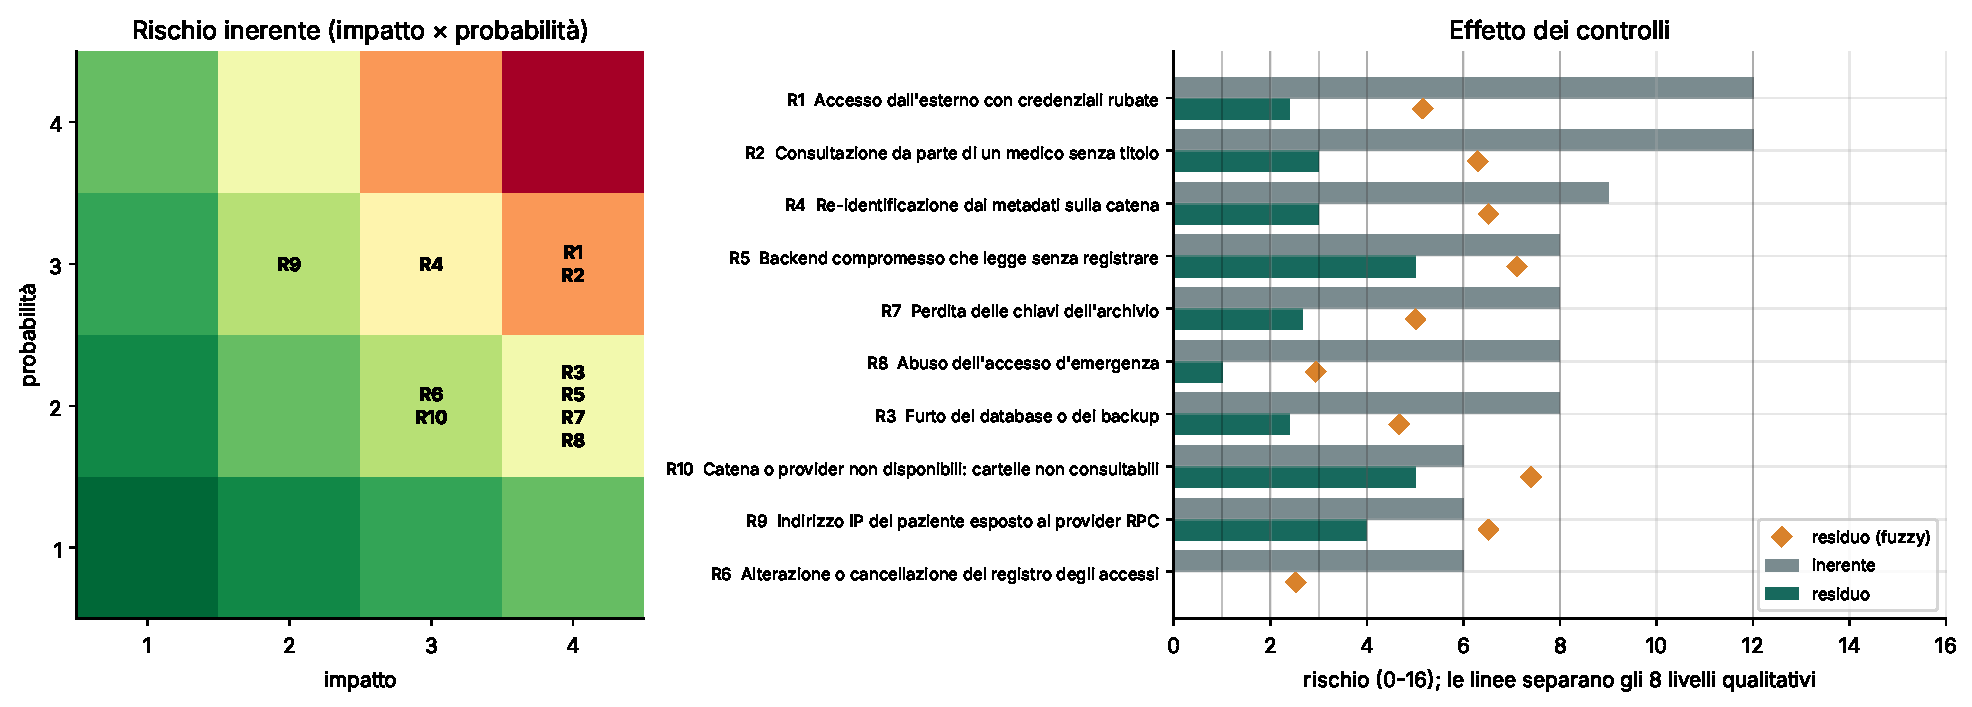
\includegraphics[width=\textwidth]{figure/dpia_rischi.pdf}
\caption{Posizione dei rischi nella matrice impatto per probabilità (a sinistra) e rischio residuo dopo i controlli, con la formula e con il sistema fuzzy (a destra).}\label{fig:dpia}
\end{figure}

I controlli tecnici abbassano di molto i rischi legati all'accesso e alla manomissione: R1, R2, R6 e R8 passano da alto o medio-alto a basso o trascurabile, grazie a passkey, consenso verificato sulla catena e registro in sola aggiunta. Restano più alti i rischi per cui il prototipo non ha ancora la contromisura, che è soprattutto organizzativa o infrastrutturale: un backend compromesso (R5), l'indisponibilità della catena (R10) e l'esposizione dell'indirizzo IP del paziente al nodo che il suo wallet interroga durante la verifica (R9). Quest'ultimo rischio è emerso proprio dalla valutazione. Il comportamento \emph{fail-closed}, scelto per non consegnare mai dati senza audit (RNF7), fa sì che un'interruzione della catena blocchi la consultazione: è il prezzo della garanzia, e va compensato con una procedura di contingenza.

\paragraph{Valutazione con la logica fuzzy.} La formula moltiplica categorie ordinali come se fossero numeri e crea salti alle soglie tra i livelli. Per controllarne la robustezza, lo stesso calcolo è ripetuto con un sistema fuzzy di Mamdani\cite{zadeh,mamdani}. Probabilità, impatto ed efficacia dei controlli sono variabili linguistiche (\emph{basso}, \emph{medio}, \emph{alto}; \emph{scarso}, \emph{parziale}, \emph{buono}) con funzioni di appartenenza triangolari. Le 27 regole, una per combinazione, partono dal livello di rischio inerente e lo abbassano di uno o due livelli secondo l'efficacia dei controlli. Le premesse si combinano con la t-norma minimo, l'uscita è ritagliata con l'implicazione di Mamdani, le regole si aggregano con il massimo e il risultato si defuzzifica con il baricentro. Il sistema fuzzy conferma l'ordine dei rischi e le stesse priorità (R10, R5, R9, R4 e R2), con valori più prudenti: il baricentro non raggiunge gli estremi della scala, e funzioni di appartenenza larghe esprimono una propensione al rischio bassa (figura~\ref{fig:fuzzy}).

\begin{figure}[H]
\centering
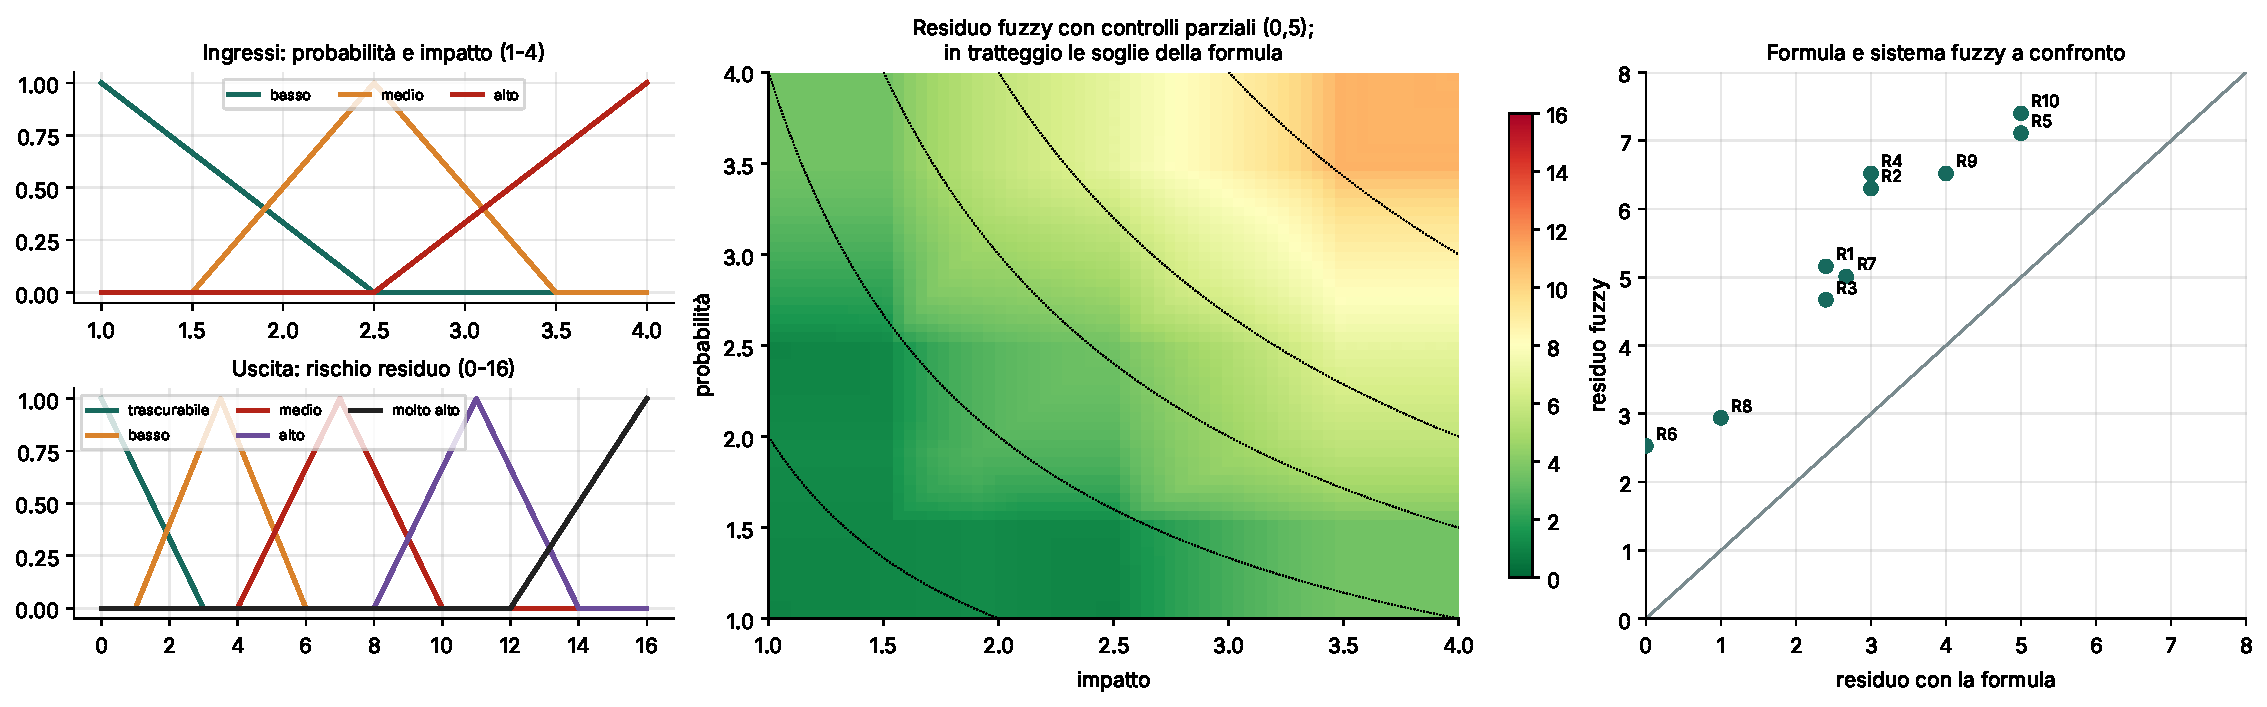
\includegraphics[width=\textwidth]{figure/dpia_fuzzy.pdf}
\caption{Sistema fuzzy: funzioni di appartenenza degli ingressi e dell'uscita (a sinistra), rischio residuo al variare di impatto e probabilità con controlli parziali, con in tratteggio le soglie della formula (al centro), e confronto tra formula e sistema fuzzy per ogni rischio (a destra).}\label{fig:fuzzy}
\end{figure}

\paragraph{Gravità di una violazione.} Per la gestione delle violazioni (artt.~33 e~34) la gravità di tre scenari è stimata con la metodologia di ENISA\cite{enisa-breach}: $SE = DPC \times EI + CB$, dove $DPC$ pesa il contesto e la natura dei dati, $EI$ la facilità di identificazione e $CB$ le circostanze della violazione (tabella~\ref{tab:enisa}).

\begin{table}[H]
\centering\footnotesize
\renewcommand{\arraystretch}{1.2}
\begin{tabular}{@{}p{.36\textwidth} ccc c l@{}}
\toprule
Scenario & $DPC$ & $EI$ & $CB$ & $SE$ & Gravità\\
\midrule
Furto del database: referti e registro (cifrati) & 4 & 0,25 & 1,0 & 2,0 & media\\
Furto del database: metadati in chiaro (nome utente del paziente, date dei referti) & 3 & 0,75 & 1,0 & 3,25 & alta\\
Furto della chiave del backend che firma le transazioni & 1 & 0,25 & 0,75 & 1,0 & bassa\\
Furto delle chiavi dell'archivio e della passphrase & 4 & 1 & 1,0 & 5,0 & molto alta\\
\bottomrule
\end{tabular}
\caption{Gravità di tre scenari di violazione. $CB$ somma la perdita di riservatezza verso destinatari ignoti (0,5) o di integrità recuperabile (0,25) e il dolo (0,5).}\label{tab:enisa}
\end{table}

Il furto del database mostra perché la valutazione va fatta sui dati e non solo sul sistema. Il contenuto clinico, cifrato con chiavi che non stanno nel database, darebbe una gravità media: la cifratura, insieme alla custodia separata delle chiavi, è una delle misure che possono esonerare dalla comunicazione agli interessati (art.~34(3)(a)). I metadati in chiaro, invece, rivelano chi è paziente della struttura e quando ha avuto un referto, e da soli rendono la violazione grave. Ne deriva una misura del piano di trattamento: sostituire nel database il nome utente del paziente con un'etichetta HMAC, come già avviene per il registro degli accessi. La chiave del backend che firma le transazioni, se rubata, permette solo di aggiungere voci false sulla catena, che il controllo sulle ricevute firmate respinge (sezione~\ref{sec:accesso}). La compromissione delle chiavi dell'archivio è lo scenario peggiore, ed è il motivo della custodia descritta nella sezione~\ref{sec:chiavi}.

\paragraph{Piano di trattamento e convalida.} Nessun rischio residuo è alto. Per quelli medi o medio-bassi il piano prevede:
\begin{itemize}
  \item \textbf{R10}: più provider del nodo in alternativa e una procedura di contingenza che consenta la consultazione d'urgenza con registrazione differita sulla catena;
  \item \textbf{R5}: chiavi dell'archivio in un modulo hardware di sicurezza e monitoraggio continuo degli eventi;
  \item \textbf{R9}: un nodo della struttura, ospitato nell'Unione europea, per le letture dal browser del paziente;
  \item \textbf{R4}: una rete \emph{permissioned} (sezione~\ref{sec:fabric}), che nasconde frequenza e orari degli accessi;
  \item \textbf{R3}: etichette HMAC al posto del nome utente nei referti, TLS verso il database e cifratura dei volumi.
\end{itemize}
Con queste misure il rischio residuo è accettabile e non serve la consultazione preventiva dell'autorità di controllo (art.~36). In un'adozione reale la valutazione andrebbe convalidata dal titolare, sentito il parere del RPD e, dove opportuno, delle rappresentanze dei pazienti (art.~35(9)). Andrebbe poi riesaminata a ogni modifica significativa del trattamento, in un ciclo di miglioramento continuo.

\subsection{Sicurezza delle reti e dei sistemi (NIS2)}\label{sec:nis2}
Come prestatore di assistenza sanitaria, la struttura è un soggetto essenziale o importante secondo le dimensioni. Le misure tecniche del sistema coprono diversi obblighi dell'art.~21 della direttiva:
\begin{itemize}
  \item autenticazione forte e resistente al phishing;
  \item crittografia, anche post-quantistica;
  \item registrazione degli eventi su un supporto non modificabile;
  \item sicurezza nello sviluppo, con revisione e campagne d'attacco;
  \item gestione delle vulnerabilità delle dipendenze;
  \item backup delle chiavi a soglia.
\end{itemize}
Restano a carico dell'organizzazione la governance, con la responsabilità degli organi di amministrazione, la formazione, la sicurezza della catena di fornitura e la continuità operativa. Per gli incidenti significativi la normativa prevede un preallarme al CSIRT nazionale entro 24 ore, una notifica entro 72 ore e una relazione finale entro un mese. Questa procedura si coordina con la notifica al Garante entro 72 ore prevista dal GDPR per le violazioni di dati personali.

\subsection{Piano di protezione dei dati}
Il piano di protezione dei dati raccoglie in un unico documento politiche, ruoli e misure che rendono operativi i principi dell'art.~5. Per il sistema ne fanno parte:
\begin{itemize}
  \item la classificazione dei dati (contenuto clinico cifrato, metadati, dati pubblici sulla catena) e il registro dei trattamenti dell'appendice~\ref{app:registro};
  \item le misure tecniche delle sezioni~\ref{sec:fido2}--\ref{sec:dati} e il piano di trattamento dei rischi qui sopra;
  \item i ruoli: RPD, custodi delle quote di backup, amministratore dei contratti, personale abilitato all'emergenza;
  \item la gestione delle violazioni, con il registro delle violazioni (art.~33(5)) e i criteri di gravità della tabella~\ref{tab:enisa};
  \item la revisione periodica degli accessi d'emergenza e la verifica annuale della valutazione d'impatto.
\end{itemize}
